\section{Digitalisierung von Signalen S. 71}
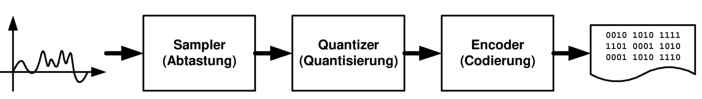
\includegraphics{content/07_digsig/digitalisierungBlockschema.pdf}
\begin{table}[H]
	\begin{tabularx}{\linewidth}{X|X}
		\begin{list}{$\bullet$}{\setlength{\itemsep}{0cm} \setlength{\parsep}{0cm}
				\setlength{\topsep}{0cm}} 
				\item Zeitdikretisierung, endliche Anzahl von Werten pro Zeit
				\item störungsfreie Übertragung
				\item Codierung (z.B. Fehlerkorrektur oder Verschlüsselung)
		\end{list}
	&
		\begin{list}{$\bullet$}{\setlength{\itemsep}{0cm} \setlength{\parsep}{0cm}
		\setlength{\topsep}{0cm}} 
			\item Quantisierung, endliche Anzahl an Amplitudenwerten (Bits)
			\item neue möglichkeiten für Signalverarbeitung
			\item Speicherung auf einheitlichen Medien
	\end{list}
	\end{tabularx}
\end{table}

\subsection{Abtastung S. 73}
\subsubsection{Ideale Abtastung S.75}
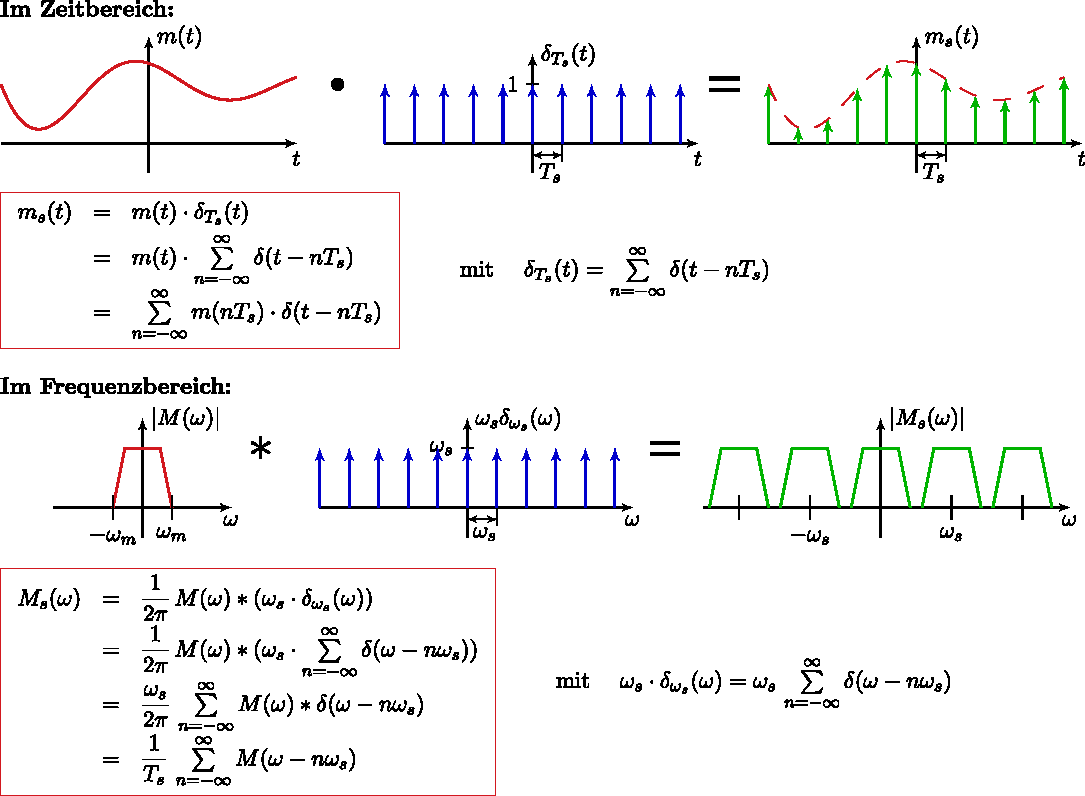
\includegraphics[width=.90\linewidth]{content/07_digsig/idealeAbtastung.pdf}

\subsubsection{Rekonstruktion mit Tiefpass S. 78}
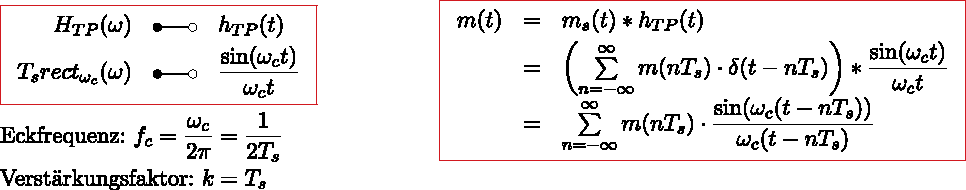
\includegraphics[width=.95\linewidth]{content/07_digsig/rekonstruktionTP.pdf}

\subsubsection{Natural Sampling S. 73}
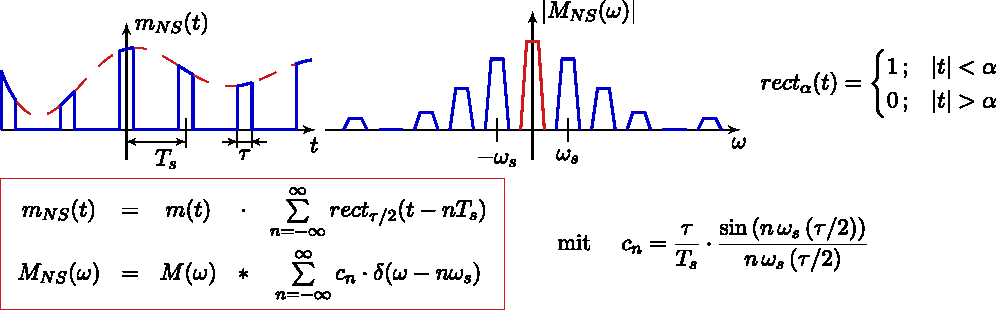
\includegraphics{content/07_digsig/naturalSampling.pdf}\\
\textbf{Rekonstruktion:} Bei der Rekonstruktion muss das Signal nach dem Tiefpass noch mit dem Faktor $\frac{T_s}{\tau}$ multipliziert werden, um die Dämpfung wieder aufzuheben.

\subsubsection{Sample {\&} Hold (ZOH), Flat-Top Sampling S. 78}
ZOH $\rightarrow$ Zero Order Hold. $H_{ZOH}(\omega) = \tau \cdot \frac{sin(\frac{\tau \omega}{2})}{\frac{\tau \omega}{2 }} \;\;\; , \;\;\; \tau \leq T_s$\\
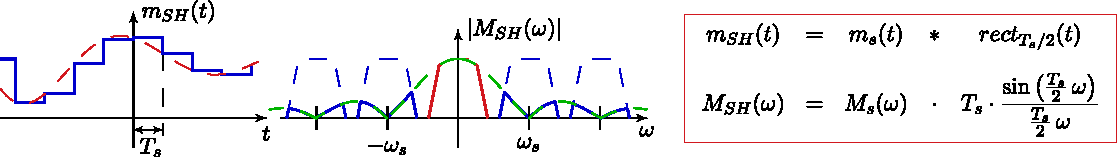
\includegraphics{content/07_digsig/flattopsampling.pdf}

\subsubsection{Nyquist-Shannon Abtasttheorem S. 76}
	\begin{list}{$\bullet$}{\setlength{\itemsep}{0cm} \setlength{\parsep}{0cm}
	\setlength{\topsep}{0cm}} 
		\item Nachrichtensignal muss auf eine Bandbreite begrenzt sein $|M(\omega)|\approx 0 \text{ für } \omega > 2\pi B_m$ (Aliasing S. 77)
		\item im Basisband darf es keine Überlappungen von Teilspektren geben, d.h. $f_s$ muss die Spektralanteile genügend weit vom ursprünglichen Spektrum wegschieben.
	\end{list}

\begin{minipage}{.3\linewidth}
	\textbf{Abtasttheorem für Basisbandsignale:} \efbox[linecolor=red]{$f_s > 2 \cdot B_m$}
\end{minipage}
\begin{minipage}{.7\linewidth}
	\begin{table}[H]
		\begin{tabularx}{\linewidth}{|m{.4\linewidth} m{.6\linewidth}}
			Nyquistrate: $f_{sN} = 2B_m$	&	Samplingfrequenz: $[f_s] = Hz$	\\
			Nyquistfrequenz: $f_N = \frac{f_s}{2}$	&	Nachrichtenfrequenz: $[f_m] = Hz$ \\
			Nyquistintervall: $T_N = \frac{1}{2B_m}$	&	Nachrichtenbandbreite: $[B_m] = Hz$\\
		\end{tabularx}
	\end{table}
\end{minipage}

\paragraph{Abtasttheroem für Bandpasssignale S. 76 (Subsampling)}
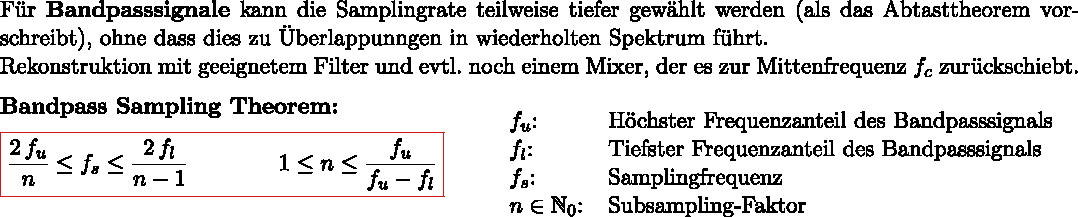
\includegraphics{content/07_digsig/subsampling.pdf}
\newpage
\paragraph{Interpolation im digitalen Bereich S. 80 (Oversampling)}
Bei Oversampling werden auf \textbf{digitaler Seite Zwischenwerte berechnet} (Interpolation) um mehr Samples zu generieren vor der D/A Wandlung. Das führt dazu, dass das \textbf{Basisband erweitert} wird (also die Blöcke im Amplitudendichtespektrum auseinandergeschoben werden, vgl Abbildung unten und "ideale Abtastung").\\
\vspace{.3cm}
Berechnung der Zwischenwerte: \efbox[linecolor=red]{$m(t)=\sum_{n=-\infty}^{\infty} m(nT_0) \frac{sin(\omega_c(t-nT_0))}{\omega_c(t-T_0)} \text{  mit  } \omega_c = \frac{\omega_s}{2}$}\\
\textbf{Vorteile:} TP-Filter kann einfacher realisiert werden (\textbf{weniger Steilheit} erforderlich), Signal wird originalgetreuer rekonstruiert; Amplitudengang des ZOH kann digital kompensiert werden.

\begin{center}
	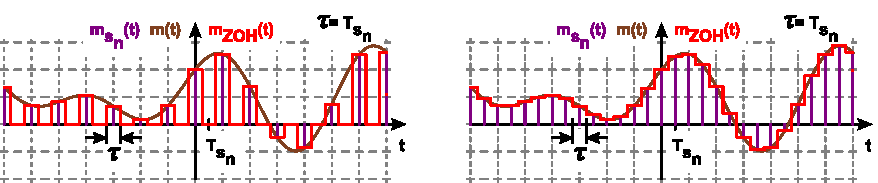
\includegraphics[width=.75\linewidth]{content/07_digsig/abbildung6_6.pdf}\\
	Zweifach interpoliertes Zero-Order Hold Signal, vor und nach dem digitalen Tiefpassfilter\\
	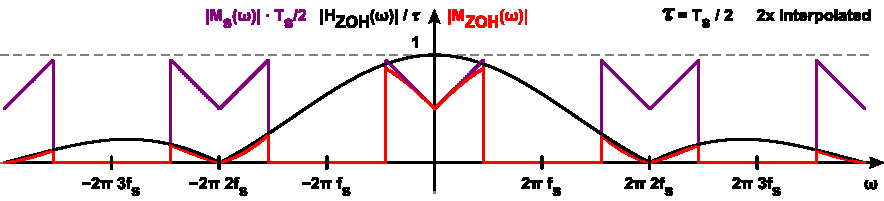
\includegraphics[width=.75\linewidth]{content/07_digsig/abbildung6_7.pdf}\\
	Zweifach interpoliertes Zero-Order Hold Signal im Frequenzbereich
\end{center}

\subsection{Quantisierung S. 81}
Nach dem Sampling liegen die zeitdiskreten Abtastwerte noch immer \textbf{amplitudenkontinuierlich} vor!
\subsubsection{Gleichförmige Quantisierung S.82}

\begin{tabularx}{\linewidth}{p{.25\linewidth} p{.2\linewidth} p{.25\linewidth} p{.2\linewidth}}
	Skalierung von $m(t)$:    & $|m_n(t) < 1$ & Wortlänge der Samples: & n Bits \\
	Quantisierungsintervalle: & $L = 2^n$     & Intervallbreite:       & $\Delta = 2/L = 2^{-(n-1)}$
\end{tabularx}\\

\paragraph{Quantisierungsrauschen}
\begin{tabularx}{\linewidth}{p{.3\textwidth} p{.65\textwidth}}
	Fehlersignal $q_e(nT)$:	& Abweichung vom effektiven Wert zum quantisierten Wert. Char. von weissem Rauschen $->$ gleichverteilt im Intervall $-\Delta/2 ... \Delta/2$\\
	Maximaler Fehler:		&  $-\Delta/2 < q_e(nT_s) < \Delta/2$ \hspace{2cm} \efbox[linecolor=red]{$P_{qe}=N=\frac{1}{\Delta} \int_{-\Delta/2}^{\Delta/2} q_e^2dq_e = \frac{\Delta^2}{12}$}
\end{tabularx}\\

\paragraph{SNR Signal-Rausch Verhältnis S. 82}
\begin{tabularx}{\linewidth}{p{.45\linewidth} p{.5\linewidth}}
	\begin{minipage}{\linewidth}
			\begin{list}{$\bullet$}{\setlength{\itemsep}{0cm} \setlength{\parsep}{0cm}
				\setlength{\topsep}{0cm}} 
			\item Signal wird maximal ausgesteuert mit\\ $|m(t)|_max = 1$
			\item $|m(t)|$ ist über Intervall $[-1...1]$ gleichverteilt
		\end{list}
	\end{minipage}
&
\begin{minipage}{\linewidth}
	\boxedeq{\begin{split} SNR_q=\frac{S}{N_q}=\frac{m^2_{RMS}}{\frac{\Delta^2}{12}} = \frac{P_m}{P_{qe}}= \frac{(\frac{1}{C})^2}{\frac{(\frac{1}{2^{n-1}})^2}{12}} = \frac{3}{C^2} \cdot 2^{2n} \\
	SNR_{q,dB} = n \cdot \qty{6.02}{\dB} + 10 \cdot log_{10} (\frac{3}{C^2}) \qty{ }{\dB} \end{split}}
\end{minipage}
\end{tabularx}

\subsubsection{Ungleichförmige Quantisierung S. 83}
	\begin{list}{$\bullet$}{\setlength{\itemsep}{0cm} \setlength{\parsep}{0cm}
		\setlength{\topsep}{0cm}} 
		\item Bei gleichförmiger Quantisierung ist N konstant $\rightarrow$ Verschlechterung der SNR bei tiefen Signalpegeln
		\item bei \textbf{Sprachsignalen vorwiegend kleine Pegel} (nicht gleichverteilt!)
		\item Quanatisierungsintervalle $\Delta$ sind für kleine Signalpegel klein und für grosse Signalpegel grösser $\rightarrow$ SNR wird verbessert
	\end{list}

\subsection{Deltamodulator S. 88}
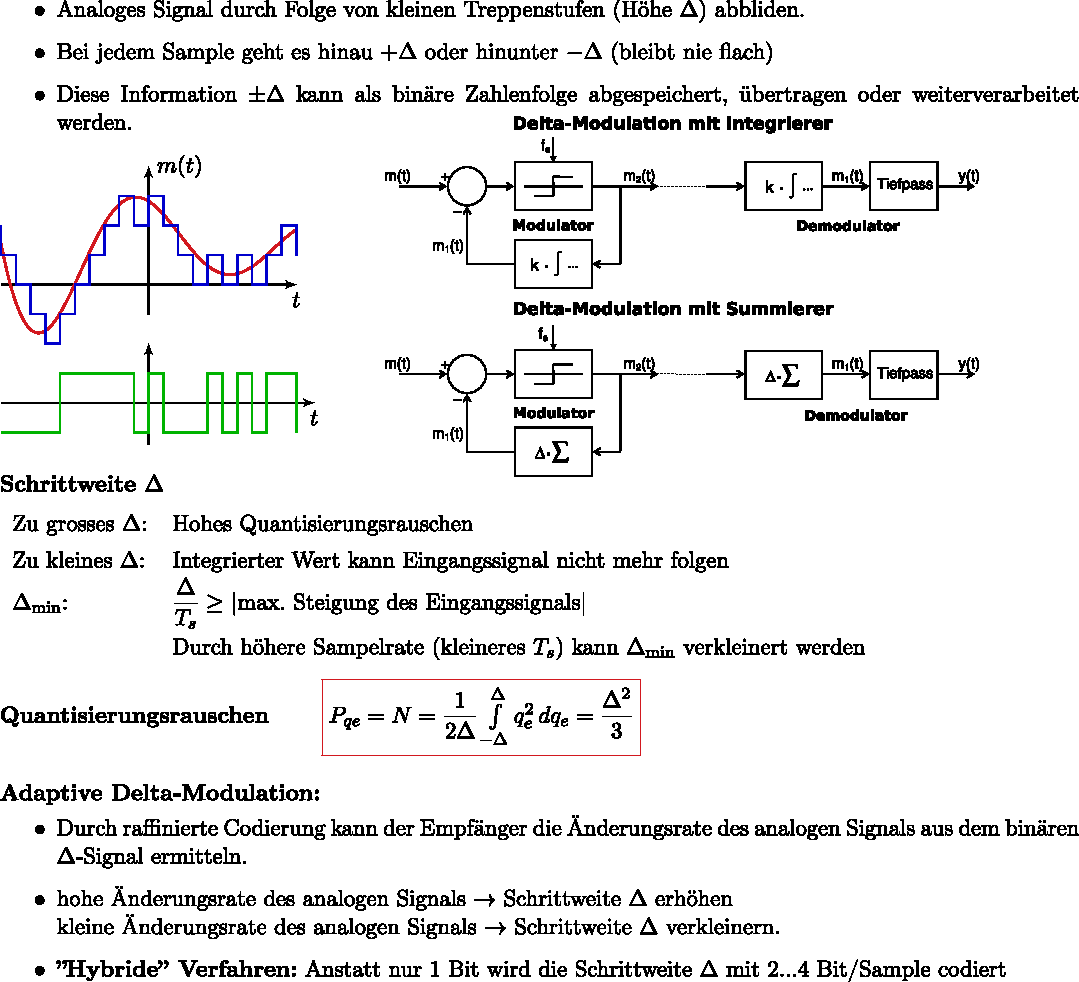
\includegraphics[width=.95\linewidth]{content/07_digsig/deltamodulator.pdf}\\
\subsection{Delta-Sigma Modulator S. 89}
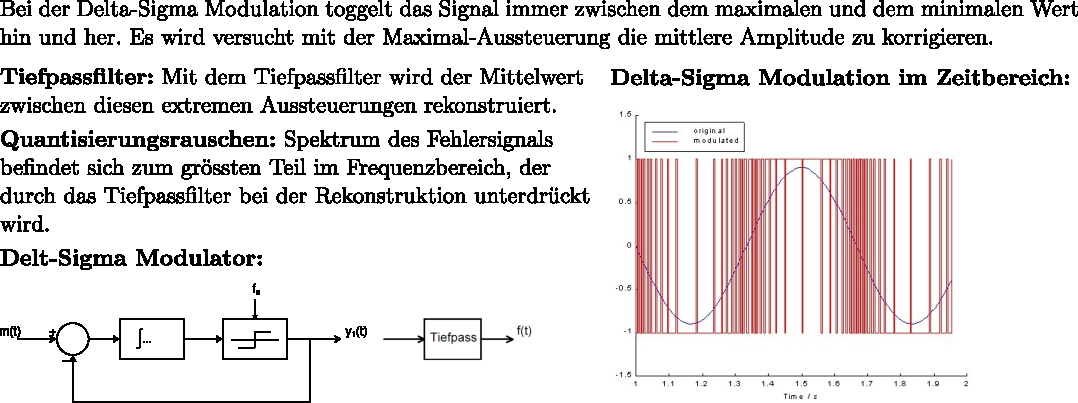
\includegraphics[width=.95\linewidth]{content/07_digsig/deltasigmamodulator.pdf}\\
